\documentclass[twoside]{book}

% Packages required by doxygen
\usepackage{fixltx2e}
\usepackage{calc}
\usepackage{doxygen}
\usepackage[export]{adjustbox} % also loads graphicx
\usepackage{graphicx}
\usepackage[utf8]{inputenc}
\usepackage{makeidx}
\usepackage{multicol}
\usepackage{multirow}
\PassOptionsToPackage{warn}{textcomp}
\usepackage{textcomp}
\usepackage[nointegrals]{wasysym}
\usepackage[table]{xcolor}

% Font selection
\usepackage[T1]{fontenc}
\usepackage[scaled=.90]{helvet}
\usepackage{courier}
\usepackage{amssymb}
\usepackage{sectsty}
\renewcommand{\familydefault}{\sfdefault}
\allsectionsfont{%
  \fontseries{bc}\selectfont%
  \color{darkgray}%
}
\renewcommand{\DoxyLabelFont}{%
  \fontseries{bc}\selectfont%
  \color{darkgray}%
}
\newcommand{\+}{\discretionary{\mbox{\scriptsize$\hookleftarrow$}}{}{}}

% Page & text layout
\usepackage{geometry}
\geometry{%
  a4paper,%
  top=2.5cm,%
  bottom=2.5cm,%
  left=2.5cm,%
  right=2.5cm%
}
\tolerance=750
\hfuzz=15pt
\hbadness=750
\setlength{\emergencystretch}{15pt}
\setlength{\parindent}{0cm}
\setlength{\parskip}{3ex plus 2ex minus 2ex}
\makeatletter
\renewcommand{\paragraph}{%
  \@startsection{paragraph}{4}{0ex}{-1.0ex}{1.0ex}{%
    \normalfont\normalsize\bfseries\SS@parafont%
  }%
}
\renewcommand{\subparagraph}{%
  \@startsection{subparagraph}{5}{0ex}{-1.0ex}{1.0ex}{%
    \normalfont\normalsize\bfseries\SS@subparafont%
  }%
}
\makeatother

% Headers & footers
\usepackage{fancyhdr}
\pagestyle{fancyplain}
\fancyhead[LE]{\fancyplain{}{\bfseries\thepage}}
\fancyhead[CE]{\fancyplain{}{}}
\fancyhead[RE]{\fancyplain{}{\bfseries\leftmark}}
\fancyhead[LO]{\fancyplain{}{\bfseries\rightmark}}
\fancyhead[CO]{\fancyplain{}{}}
\fancyhead[RO]{\fancyplain{}{\bfseries\thepage}}
\fancyfoot[LE]{\fancyplain{}{}}
\fancyfoot[CE]{\fancyplain{}{}}
\fancyfoot[RE]{\fancyplain{}{\bfseries\scriptsize Generated by Doxygen }}
\fancyfoot[LO]{\fancyplain{}{\bfseries\scriptsize Generated by Doxygen }}
\fancyfoot[CO]{\fancyplain{}{}}
\fancyfoot[RO]{\fancyplain{}{}}
\renewcommand{\footrulewidth}{0.4pt}
\renewcommand{\chaptermark}[1]{%
  \markboth{#1}{}%
}
\renewcommand{\sectionmark}[1]{%
  \markright{\thesection\ #1}%
}

% Indices & bibliography
\usepackage{natbib}
\usepackage[titles]{tocloft}
\setcounter{tocdepth}{3}
\setcounter{secnumdepth}{5}
\makeindex

% Hyperlinks (required, but should be loaded last)
\usepackage{ifpdf}
\ifpdf
  \usepackage[pdftex,pagebackref=true]{hyperref}
\else
  \usepackage[ps2pdf,pagebackref=true]{hyperref}
\fi
\hypersetup{%
  colorlinks=true,%
  linkcolor=blue,%
  citecolor=blue,%
  unicode%
}

% Custom commands
\newcommand{\clearemptydoublepage}{%
  \newpage{\pagestyle{empty}\cleardoublepage}%
}

\usepackage{caption}
\captionsetup{labelsep=space,justification=centering,font={bf},singlelinecheck=off,skip=4pt,position=top}

%===== C O N T E N T S =====

\begin{document}

% Titlepage & ToC
\hypersetup{pageanchor=false,
             bookmarksnumbered=true,
             pdfencoding=unicode
            }
\pagenumbering{alph}
\begin{titlepage}
\vspace*{7cm}
\begin{center}%
{\Large Proc Control \\[1ex]\large 1.\+0 }\\
\vspace*{1cm}
{\large Generated by Doxygen 1.8.13}\\
\end{center}
\end{titlepage}
\clearemptydoublepage
\pagenumbering{roman}
\tableofcontents
\clearemptydoublepage
\pagenumbering{arabic}
\hypersetup{pageanchor=true}

%--- Begin generated contents ---
\chapter{Class Index}
\section{Class List}
Here are the classes, structs, unions and interfaces with brief descriptions\+:\begin{DoxyCompactList}
\item\contentsline{section}{\hyperlink{classproc__control_1_1_proc_control_node}{proc\+\_\+control\+::\+Proc\+Control\+Node} }{\pageref{classproc__control_1_1_proc_control_node}}{}
\end{DoxyCompactList}

\chapter{File Index}
\section{File List}
Here is a list of all documented files with brief descriptions\+:\begin{DoxyCompactList}
\item\contentsline{section}{\hyperlink{main_8cc}{main.\+cc} }{\pageref{main_8cc}}{}
\item\contentsline{section}{\hyperlink{proc__control__node_8cc}{proc\+\_\+control\+\_\+node.\+cc} }{\pageref{proc__control__node_8cc}}{}
\item\contentsline{section}{\hyperlink{proc__control__node_8h}{proc\+\_\+control\+\_\+node.\+h} }{\pageref{proc__control__node_8h}}{}
\item\contentsline{section}{\hyperlink{property_8h}{property.\+h} }{\pageref{property_8h}}{}
\end{DoxyCompactList}

\chapter{Class Documentation}
\hypertarget{classproc__control_1_1_proc_control_node}{}\section{proc\+\_\+control\+:\+:Proc\+Control\+Node Class Reference}
\label{classproc__control_1_1_proc_control_node}\index{proc\+\_\+control\+::\+Proc\+Control\+Node@{proc\+\_\+control\+::\+Proc\+Control\+Node}}
\subsection*{Public Member Functions}
\begin{DoxyCompactItemize}
\item 
\hyperlink{classproc__control_1_1_proc_control_node_a3990253ca2e924c15e25cecba4297359}{Proc\+Control\+Node} (const ros\+::\+Node\+Handle\+Ptr \&nh)
\item 
\hyperlink{classproc__control_1_1_proc_control_node_ac4ec58d30c4c8a5842f1797154b6e363}{$\sim$\+Proc\+Control\+Node} ()
\item 
void \hyperlink{classproc__control_1_1_proc_control_node_adc8a2178d41c620f69cb74c2f09097cd}{Control\+Loop} ()
\item 
bool \hyperlink{classproc__control_1_1_proc_control_node_ac56aa1e6e028c225be157371aba76d32}{Set\+Control\+Mode\+Callback} (proc\+\_\+control\+::\+Set\+Control\+Mode\+Request \&request, proc\+\_\+control\+::\+Set\+Control\+Mode\+Response \&response)
\item 
bool \hyperlink{classproc__control_1_1_proc_control_node_a7890db7144358d5aaf0daa7bfefed964}{Set\+Global\+Target\+Position\+Callback} (proc\+\_\+control\+::\+Set\+Position\+Target\+Request \&request, proc\+\_\+control\+::\+Set\+Position\+Target\+Response \&response)
\item 
bool \hyperlink{classproc__control_1_1_proc_control_node_ad331887883a3c1c44472d72dfced3db6}{Set\+Local\+Target\+Position\+Callback} (proc\+\_\+control\+::\+Set\+Position\+Target\+Request \&request, proc\+\_\+control\+::\+Set\+Position\+Target\+Response \&response)
\item 
bool \hyperlink{classproc__control_1_1_proc_control_node_a841b03177a02e542bf7f7aa8403c5382}{Set\+Global\+Decoupled\+Target\+Position\+Callback} (proc\+\_\+control\+::\+Set\+Decoupled\+Target\+Request \&request, proc\+\_\+control\+::\+Set\+Decoupled\+Target\+Response \&response)
\item 
bool \hyperlink{classproc__control_1_1_proc_control_node_a01301ec4fcd9e4d149994cbe27ff8ca1}{Set\+Local\+Decoupled\+Target\+Position\+Callback} (proc\+\_\+control\+::\+Set\+Decoupled\+Target\+Request \&request, proc\+\_\+control\+::\+Set\+Decoupled\+Target\+Response \&response)
\end{DoxyCompactItemize}
\subsection*{Public Attributes}
\begin{DoxyCompactItemize}
\item 
\mbox{\Hypertarget{classproc__control_1_1_proc_control_node_a5e3562edaa6eba1d9bf3cc9b17afbd8a}\label{classproc__control_1_1_proc_control_node_a5e3562edaa6eba1d9bf3cc9b17afbd8a}} 
const bool {\bfseries Global\+Target} = true
\item 
\mbox{\Hypertarget{classproc__control_1_1_proc_control_node_a9de14df77c66166cfaaaefa31726ea00}\label{classproc__control_1_1_proc_control_node_a9de14df77c66166cfaaaefa31726ea00}} 
const bool {\bfseries Local\+Target} = false
\end{DoxyCompactItemize}


\subsection{Constructor \& Destructor Documentation}
\mbox{\Hypertarget{classproc__control_1_1_proc_control_node_a3990253ca2e924c15e25cecba4297359}\label{classproc__control_1_1_proc_control_node_a3990253ca2e924c15e25cecba4297359}} 
\index{proc\+\_\+control\+::\+Proc\+Control\+Node@{proc\+\_\+control\+::\+Proc\+Control\+Node}!Proc\+Control\+Node@{Proc\+Control\+Node}}
\index{Proc\+Control\+Node@{Proc\+Control\+Node}!proc\+\_\+control\+::\+Proc\+Control\+Node@{proc\+\_\+control\+::\+Proc\+Control\+Node}}
\subsubsection{\texorpdfstring{Proc\+Control\+Node()}{ProcControlNode()}}
{\footnotesize\ttfamily proc\+\_\+control\+::\+Proc\+Control\+Node\+::\+Proc\+Control\+Node (\begin{DoxyParamCaption}\item[{const ros\+::\+Node\+Handle\+Ptr \&}]{nh }\end{DoxyParamCaption})}

Constructor of the \hyperlink{classproc__control_1_1_proc_control_node}{Proc\+Control\+Node} object. 
\begin{DoxyParams}{Parameters}
{\em nh} & Node handler pointer. \\
\hline
\end{DoxyParams}
\mbox{\Hypertarget{classproc__control_1_1_proc_control_node_ac4ec58d30c4c8a5842f1797154b6e363}\label{classproc__control_1_1_proc_control_node_ac4ec58d30c4c8a5842f1797154b6e363}} 
\index{proc\+\_\+control\+::\+Proc\+Control\+Node@{proc\+\_\+control\+::\+Proc\+Control\+Node}!````~Proc\+Control\+Node@{$\sim$\+Proc\+Control\+Node}}
\index{````~Proc\+Control\+Node@{$\sim$\+Proc\+Control\+Node}!proc\+\_\+control\+::\+Proc\+Control\+Node@{proc\+\_\+control\+::\+Proc\+Control\+Node}}
\subsubsection{\texorpdfstring{$\sim$\+Proc\+Control\+Node()}{~ProcControlNode()}}
{\footnotesize\ttfamily proc\+\_\+control\+::\+Proc\+Control\+Node\+::$\sim$\+Proc\+Control\+Node (\begin{DoxyParamCaption}{ }\end{DoxyParamCaption})}

Destructor of the \hyperlink{classproc__control_1_1_proc_control_node}{Proc\+Control\+Node} object. Shutdown all the connections to the services needed. 

\subsection{Member Function Documentation}
\mbox{\Hypertarget{classproc__control_1_1_proc_control_node_adc8a2178d41c620f69cb74c2f09097cd}\label{classproc__control_1_1_proc_control_node_adc8a2178d41c620f69cb74c2f09097cd}} 
\index{proc\+\_\+control\+::\+Proc\+Control\+Node@{proc\+\_\+control\+::\+Proc\+Control\+Node}!Control\+Loop@{Control\+Loop}}
\index{Control\+Loop@{Control\+Loop}!proc\+\_\+control\+::\+Proc\+Control\+Node@{proc\+\_\+control\+::\+Proc\+Control\+Node}}
\subsubsection{\texorpdfstring{Control\+Loop()}{ControlLoop()}}
{\footnotesize\ttfamily void proc\+\_\+control\+::\+Proc\+Control\+Node\+::\+Control\+Loop (\begin{DoxyParamCaption}{ }\end{DoxyParamCaption})}

A simple function that set \hyperlink{classproc__control_1_1_robot_state}{Robot\+State} from input and process position mode. \mbox{\Hypertarget{classproc__control_1_1_proc_control_node_ac56aa1e6e028c225be157371aba76d32}\label{classproc__control_1_1_proc_control_node_ac56aa1e6e028c225be157371aba76d32}} 
\index{proc\+\_\+control\+::\+Proc\+Control\+Node@{proc\+\_\+control\+::\+Proc\+Control\+Node}!Set\+Control\+Mode\+Callback@{Set\+Control\+Mode\+Callback}}
\index{Set\+Control\+Mode\+Callback@{Set\+Control\+Mode\+Callback}!proc\+\_\+control\+::\+Proc\+Control\+Node@{proc\+\_\+control\+::\+Proc\+Control\+Node}}
\subsubsection{\texorpdfstring{Set\+Control\+Mode\+Callback()}{SetControlModeCallback()}}
{\footnotesize\ttfamily bool proc\+\_\+control\+::\+Proc\+Control\+Node\+::\+Set\+Control\+Mode\+Callback (\begin{DoxyParamCaption}\item[{proc\+\_\+control\+::\+Set\+Control\+Mode\+Request \&}]{request,  }\item[{proc\+\_\+control\+::\+Set\+Control\+Mode\+Response \&}]{response }\end{DoxyParamCaption})}

Callback used to change the control mode \+: position or P\+PI or speed. 
\begin{DoxyParams}{Parameters}
{\em request} & The new control mode requested (request.\+mode). \\
\hline
{\em response} & This parameter isn\textquotesingle{}t use. \\
\hline
\end{DoxyParams}
\begin{DoxyReturn}{Returns}
true 
\end{DoxyReturn}
\mbox{\Hypertarget{classproc__control_1_1_proc_control_node_a841b03177a02e542bf7f7aa8403c5382}\label{classproc__control_1_1_proc_control_node_a841b03177a02e542bf7f7aa8403c5382}} 
\index{proc\+\_\+control\+::\+Proc\+Control\+Node@{proc\+\_\+control\+::\+Proc\+Control\+Node}!Set\+Global\+Decoupled\+Target\+Position\+Callback@{Set\+Global\+Decoupled\+Target\+Position\+Callback}}
\index{Set\+Global\+Decoupled\+Target\+Position\+Callback@{Set\+Global\+Decoupled\+Target\+Position\+Callback}!proc\+\_\+control\+::\+Proc\+Control\+Node@{proc\+\_\+control\+::\+Proc\+Control\+Node}}
\subsubsection{\texorpdfstring{Set\+Global\+Decoupled\+Target\+Position\+Callback()}{SetGlobalDecoupledTargetPositionCallback()}}
{\footnotesize\ttfamily bool proc\+\_\+control\+::\+Proc\+Control\+Node\+::\+Set\+Global\+Decoupled\+Target\+Position\+Callback (\begin{DoxyParamCaption}\item[{proc\+\_\+control\+::\+Set\+Decoupled\+Target\+Request \&}]{request,  }\item[{proc\+\_\+control\+::\+Set\+Decoupled\+Target\+Response \&}]{response }\end{DoxyParamCaption})}

Callback used to set global decoupled target position. 
\begin{DoxyParams}{Parameters}
{\em request} & The new global decoupled target position requested (request.\+X, request.\+Y, request.\+Z, request.\+Y\+AW, request.\+R\+O\+LL, request.\+P\+I\+T\+CH, request.\+keepX, request.\+keepY, request.\+keepZ, request.\+keep\+R\+O\+LL, request.\+keep\+P\+I\+T\+CH, request.\+keep\+Y\+AW) \\
\hline
{\em response} & This parameter isn\textquotesingle{}t use. \\
\hline
\end{DoxyParams}
\begin{DoxyReturn}{Returns}
true 
\end{DoxyReturn}
\mbox{\Hypertarget{classproc__control_1_1_proc_control_node_a7890db7144358d5aaf0daa7bfefed964}\label{classproc__control_1_1_proc_control_node_a7890db7144358d5aaf0daa7bfefed964}} 
\index{proc\+\_\+control\+::\+Proc\+Control\+Node@{proc\+\_\+control\+::\+Proc\+Control\+Node}!Set\+Global\+Target\+Position\+Callback@{Set\+Global\+Target\+Position\+Callback}}
\index{Set\+Global\+Target\+Position\+Callback@{Set\+Global\+Target\+Position\+Callback}!proc\+\_\+control\+::\+Proc\+Control\+Node@{proc\+\_\+control\+::\+Proc\+Control\+Node}}
\subsubsection{\texorpdfstring{Set\+Global\+Target\+Position\+Callback()}{SetGlobalTargetPositionCallback()}}
{\footnotesize\ttfamily bool proc\+\_\+control\+::\+Proc\+Control\+Node\+::\+Set\+Global\+Target\+Position\+Callback (\begin{DoxyParamCaption}\item[{proc\+\_\+control\+::\+Set\+Position\+Target\+Request \&}]{request,  }\item[{proc\+\_\+control\+::\+Set\+Position\+Target\+Response \&}]{response }\end{DoxyParamCaption})}

Callback used to set global target position. 
\begin{DoxyParams}{Parameters}
{\em request} & The new global target position requested (request.\+X, request.\+Y, request.\+Z, request.\+Y\+AW, request.\+R\+O\+LL, request.\+P\+I\+T\+CH). \\
\hline
{\em response} & This parameter isn\textquotesingle{}t use. \\
\hline
\end{DoxyParams}
\begin{DoxyReturn}{Returns}
true 
\end{DoxyReturn}
\mbox{\Hypertarget{classproc__control_1_1_proc_control_node_a01301ec4fcd9e4d149994cbe27ff8ca1}\label{classproc__control_1_1_proc_control_node_a01301ec4fcd9e4d149994cbe27ff8ca1}} 
\index{proc\+\_\+control\+::\+Proc\+Control\+Node@{proc\+\_\+control\+::\+Proc\+Control\+Node}!Set\+Local\+Decoupled\+Target\+Position\+Callback@{Set\+Local\+Decoupled\+Target\+Position\+Callback}}
\index{Set\+Local\+Decoupled\+Target\+Position\+Callback@{Set\+Local\+Decoupled\+Target\+Position\+Callback}!proc\+\_\+control\+::\+Proc\+Control\+Node@{proc\+\_\+control\+::\+Proc\+Control\+Node}}
\subsubsection{\texorpdfstring{Set\+Local\+Decoupled\+Target\+Position\+Callback()}{SetLocalDecoupledTargetPositionCallback()}}
{\footnotesize\ttfamily bool proc\+\_\+control\+::\+Proc\+Control\+Node\+::\+Set\+Local\+Decoupled\+Target\+Position\+Callback (\begin{DoxyParamCaption}\item[{proc\+\_\+control\+::\+Set\+Decoupled\+Target\+Request \&}]{request,  }\item[{proc\+\_\+control\+::\+Set\+Decoupled\+Target\+Response \&}]{response }\end{DoxyParamCaption})}

Callback used to set local decoupled target position. 
\begin{DoxyParams}{Parameters}
{\em request} & The new global decoupled target position requested (request.\+X, request.\+Y, request.\+Z, request.\+Y\+AW, request.\+R\+O\+LL, request.\+P\+I\+T\+CH, request.\+keepX, request.\+keepY, request.\+keepZ, request.\+keep\+R\+O\+LL, request.\+keep\+P\+I\+T\+CH, request.\+keep\+Y\+AW) \\
\hline
{\em response} & This parameter isn\textquotesingle{}t use. \\
\hline
\end{DoxyParams}
\begin{DoxyReturn}{Returns}
true 
\end{DoxyReturn}
\mbox{\Hypertarget{classproc__control_1_1_proc_control_node_ad331887883a3c1c44472d72dfced3db6}\label{classproc__control_1_1_proc_control_node_ad331887883a3c1c44472d72dfced3db6}} 
\index{proc\+\_\+control\+::\+Proc\+Control\+Node@{proc\+\_\+control\+::\+Proc\+Control\+Node}!Set\+Local\+Target\+Position\+Callback@{Set\+Local\+Target\+Position\+Callback}}
\index{Set\+Local\+Target\+Position\+Callback@{Set\+Local\+Target\+Position\+Callback}!proc\+\_\+control\+::\+Proc\+Control\+Node@{proc\+\_\+control\+::\+Proc\+Control\+Node}}
\subsubsection{\texorpdfstring{Set\+Local\+Target\+Position\+Callback()}{SetLocalTargetPositionCallback()}}
{\footnotesize\ttfamily bool proc\+\_\+control\+::\+Proc\+Control\+Node\+::\+Set\+Local\+Target\+Position\+Callback (\begin{DoxyParamCaption}\item[{proc\+\_\+control\+::\+Set\+Position\+Target\+Request \&}]{request,  }\item[{proc\+\_\+control\+::\+Set\+Position\+Target\+Response \&}]{response }\end{DoxyParamCaption})}

Callback used to set local target position. 
\begin{DoxyParams}{Parameters}
{\em request} & The new local target position requested (request.\+X, request.\+Y, request.\+Z, request.\+Y\+AW, request.\+R\+O\+LL, request.\+P\+I\+T\+CH). \\
\hline
{\em response} & This parameter isn\textquotesingle{}t use. \\
\hline
\end{DoxyParams}
\begin{DoxyReturn}{Returns}
true 
\end{DoxyReturn}


The documentation for this class was generated from the following files\+:\begin{DoxyCompactItemize}
\item 
\hyperlink{proc__control__node_8h}{proc\+\_\+control\+\_\+node.\+h}\item 
\hyperlink{proc__control__node_8cc}{proc\+\_\+control\+\_\+node.\+cc}\end{DoxyCompactItemize}

\chapter{File Documentation}
\hypertarget{main_8cc}{}\section{main.\+cc File Reference}
\label{main_8cc}\index{main.\+cc@{main.\+cc}}
{\ttfamily \#include $<$ros/ros.\+h$>$}\newline
{\ttfamily \#include \char`\"{}proc\+\_\+control\+\_\+node.\+h\char`\"{}}\newline
Include dependency graph for main.\+cc\+:\nopagebreak
\begin{figure}[H]
\begin{center}
\leavevmode
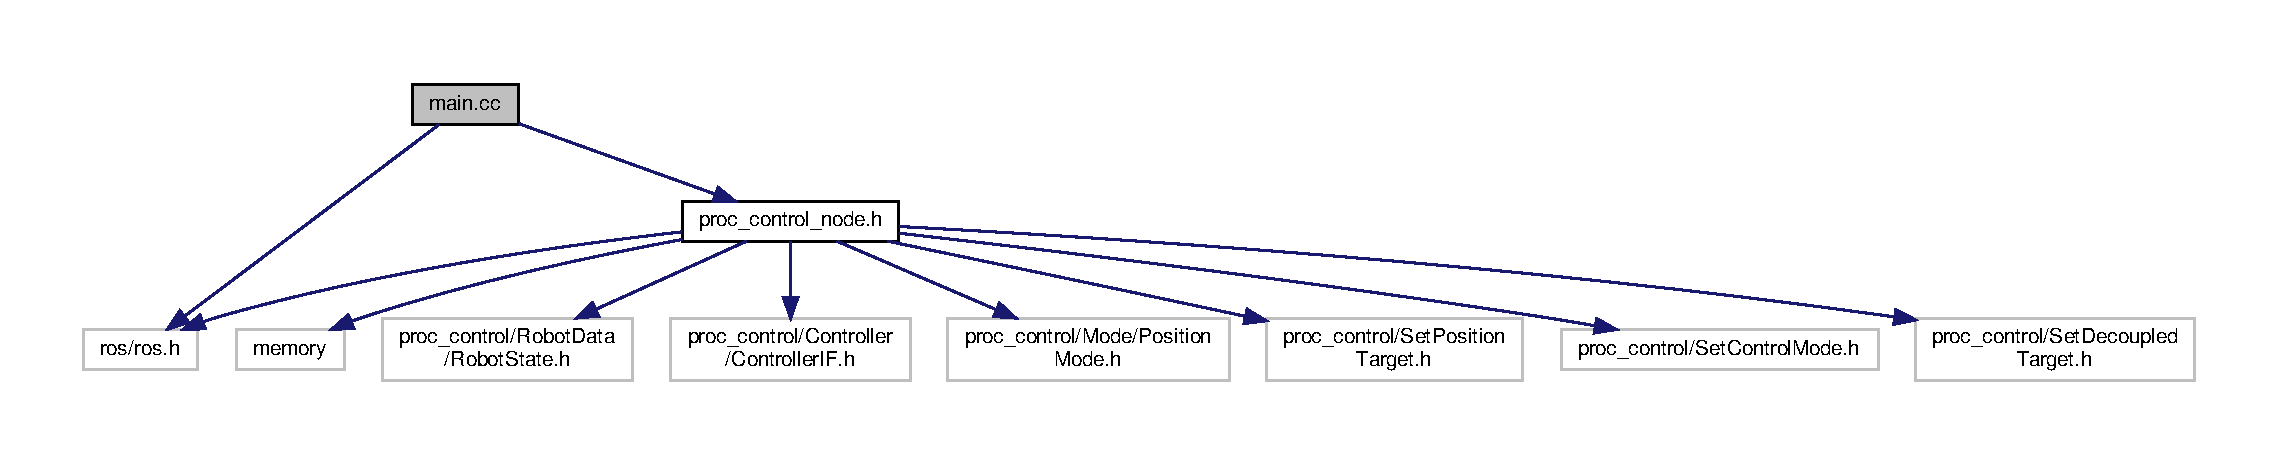
\includegraphics[width=350pt]{main_8cc__incl}
\end{center}
\end{figure}
\subsection*{Functions}
\begin{DoxyCompactItemize}
\item 
\mbox{\Hypertarget{main_8cc_a3c04138a5bfe5d72780bb7e82a18e627}\label{main_8cc_a3c04138a5bfe5d72780bb7e82a18e627}} 
int {\bfseries main} (int argc, char $\ast$$\ast$argv)
\end{DoxyCompactItemize}


\subsection{Detailed Description}
\begin{DoxyAuthor}{Author}
Jeremie St-\/\+Jules-\/\+Prevost \href{mailto:jeremie.st.jules.prevost@gmail.com}{\tt jeremie.\+st.\+jules.\+prevost@gmail.\+com} 
\end{DoxyAuthor}
\begin{DoxyDate}{Date}
24/01/2016
\end{DoxyDate}
\begin{DoxyCopyright}{Copyright}
Copyright (c) 2017 S.\+O.\+N.\+I.\+A. All rights reserved.
\end{DoxyCopyright}
This file contains the main function of proc control.\hypertarget{property_8h_LICENSE}{}\subsection{L\+I\+C\+E\+N\+SE}\label{property_8h_LICENSE}
This file is part of S.\+O.\+N.\+I.\+A. A\+UV software.

S.\+O.\+N.\+I.\+A. A\+UV software is free software\+: you can redistribute it and/or modify it under the terms of the G\+NU General Public License as published by the Free Software Foundation, either version 3 of the License, or (at your option) any later version.

S.\+O.\+N.\+I.\+A. A\+UV software is distributed in the hope that it will be useful, but W\+I\+T\+H\+O\+UT A\+NY W\+A\+R\+R\+A\+N\+TY; without even the implied warranty of M\+E\+R\+C\+H\+A\+N\+T\+A\+B\+I\+L\+I\+TY or F\+I\+T\+N\+E\+SS F\+OR A P\+A\+R\+T\+I\+C\+U\+L\+AR P\+U\+R\+P\+O\+SE. See the G\+NU General Public License for more details.

You should have received a copy of the G\+NU General Public License along with S.\+O.\+N.\+I.\+A. A\+UV software. If not, see \href{http://www.gnu.org/licenses/}{\tt http\+://www.\+gnu.\+org/licenses/}. 
\hypertarget{proc__control__node_8cc}{}\section{proc\+\_\+control\+\_\+node.\+cc File Reference}
\label{proc__control__node_8cc}\index{proc\+\_\+control\+\_\+node.\+cc@{proc\+\_\+control\+\_\+node.\+cc}}
{\ttfamily \#include \char`\"{}proc\+\_\+control\+\_\+node.\+h\char`\"{}}\newline
{\ttfamily \#include \char`\"{}proc\+\_\+control/\+Mode/\+Velocity\+Mode.\+h\char`\"{}}\newline
{\ttfamily \#include \char`\"{}proc\+\_\+control/\+Controller/\+P\+I\+D\+Controller.\+h\char`\"{}}\newline
{\ttfamily \#include \char`\"{}proc\+\_\+control/\+Controller/\+P\+P\+I\+Controller.\+h\char`\"{}}\newline
{\ttfamily \#include \char`\"{}proc\+\_\+control/\+Controller/\+B\+Controller.\+h\char`\"{}}\newline
Include dependency graph for proc\+\_\+control\+\_\+node.\+cc\+:\nopagebreak
\begin{figure}[H]
\begin{center}
\leavevmode
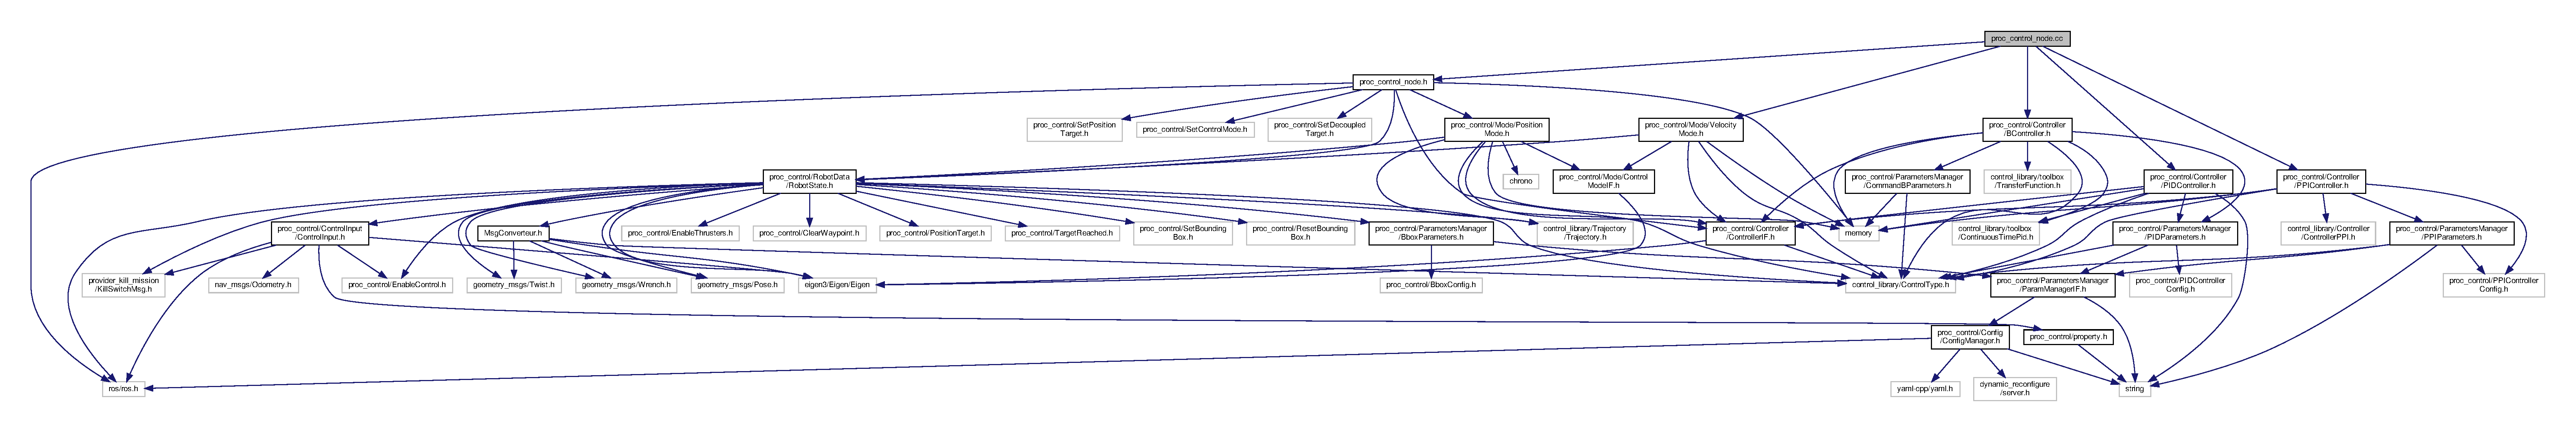
\includegraphics[width=350pt]{proc__control__node_8cc__incl}
\end{center}
\end{figure}


\subsection{Detailed Description}
\begin{DoxyAuthor}{Author}
Olivier Lavoie \href{mailto:olavoie9507@gmail.com}{\tt olavoie9507@gmail.\+com} 
\end{DoxyAuthor}
\begin{DoxyDate}{Date}
10/21/17
\end{DoxyDate}
\begin{DoxyCopyright}{Copyright}
Copyright (c) 2017 S.\+O.\+N.\+I.\+A. A\+UV All rights reserved.
\end{DoxyCopyright}
This file contains the proc control node code.\hypertarget{_robot_state_8h_LICENSE}{}\subsection{L\+I\+C\+E\+N\+SE}\label{_robot_state_8h_LICENSE}
This file is part of S.\+O.\+N.\+I.\+A. software.

S.\+O.\+N.\+I.\+A. A\+UV software is free software\+: you can redistribute it and/or modify it under the terms of the G\+NU General Public License as published by the Free Software Foundation, either version 3 of the License, or (at your option) any later version.

S.\+O.\+N.\+I.\+A. A\+UV software is distributed in the hope that it will be useful, but W\+I\+T\+H\+O\+UT A\+NY W\+A\+R\+R\+A\+N\+TY; without even the implied warranty of M\+E\+R\+C\+H\+A\+N\+T\+A\+B\+I\+L\+I\+TY or F\+I\+T\+N\+E\+SS F\+OR A P\+A\+R\+T\+I\+C\+U\+L\+AR P\+U\+R\+P\+O\+SE. See the G\+NU General Public License for more details.

You should have received a copy of the G\+NU General Public License along with S.\+O.\+N.\+I.\+A. A\+UV software. If not, see \href{http://www.gnu.org/licenses/}{\tt http\+://www.\+gnu.\+org/licenses/}. 
\hypertarget{proc__control__node_8h}{}\section{proc\+\_\+control\+\_\+node.\+h File Reference}
\label{proc__control__node_8h}\index{proc\+\_\+control\+\_\+node.\+h@{proc\+\_\+control\+\_\+node.\+h}}
{\ttfamily \#include $<$ros/ros.\+h$>$}\newline
{\ttfamily \#include $<$memory$>$}\newline
{\ttfamily \#include \char`\"{}proc\+\_\+control/\+Robot\+Data/\+Robot\+State.\+h\char`\"{}}\newline
{\ttfamily \#include \char`\"{}proc\+\_\+control/\+Controller/\+Controller\+I\+F.\+h\char`\"{}}\newline
{\ttfamily \#include \char`\"{}proc\+\_\+control/\+Mode/\+Position\+Mode.\+h\char`\"{}}\newline
{\ttfamily \#include \char`\"{}proc\+\_\+control/\+Set\+Position\+Target.\+h\char`\"{}}\newline
{\ttfamily \#include \char`\"{}proc\+\_\+control/\+Set\+Control\+Mode.\+h\char`\"{}}\newline
{\ttfamily \#include \char`\"{}proc\+\_\+control/\+Set\+Decoupled\+Target.\+h\char`\"{}}\newline
Include dependency graph for proc\+\_\+control\+\_\+node.\+h\+:\nopagebreak
\begin{figure}[H]
\begin{center}
\leavevmode
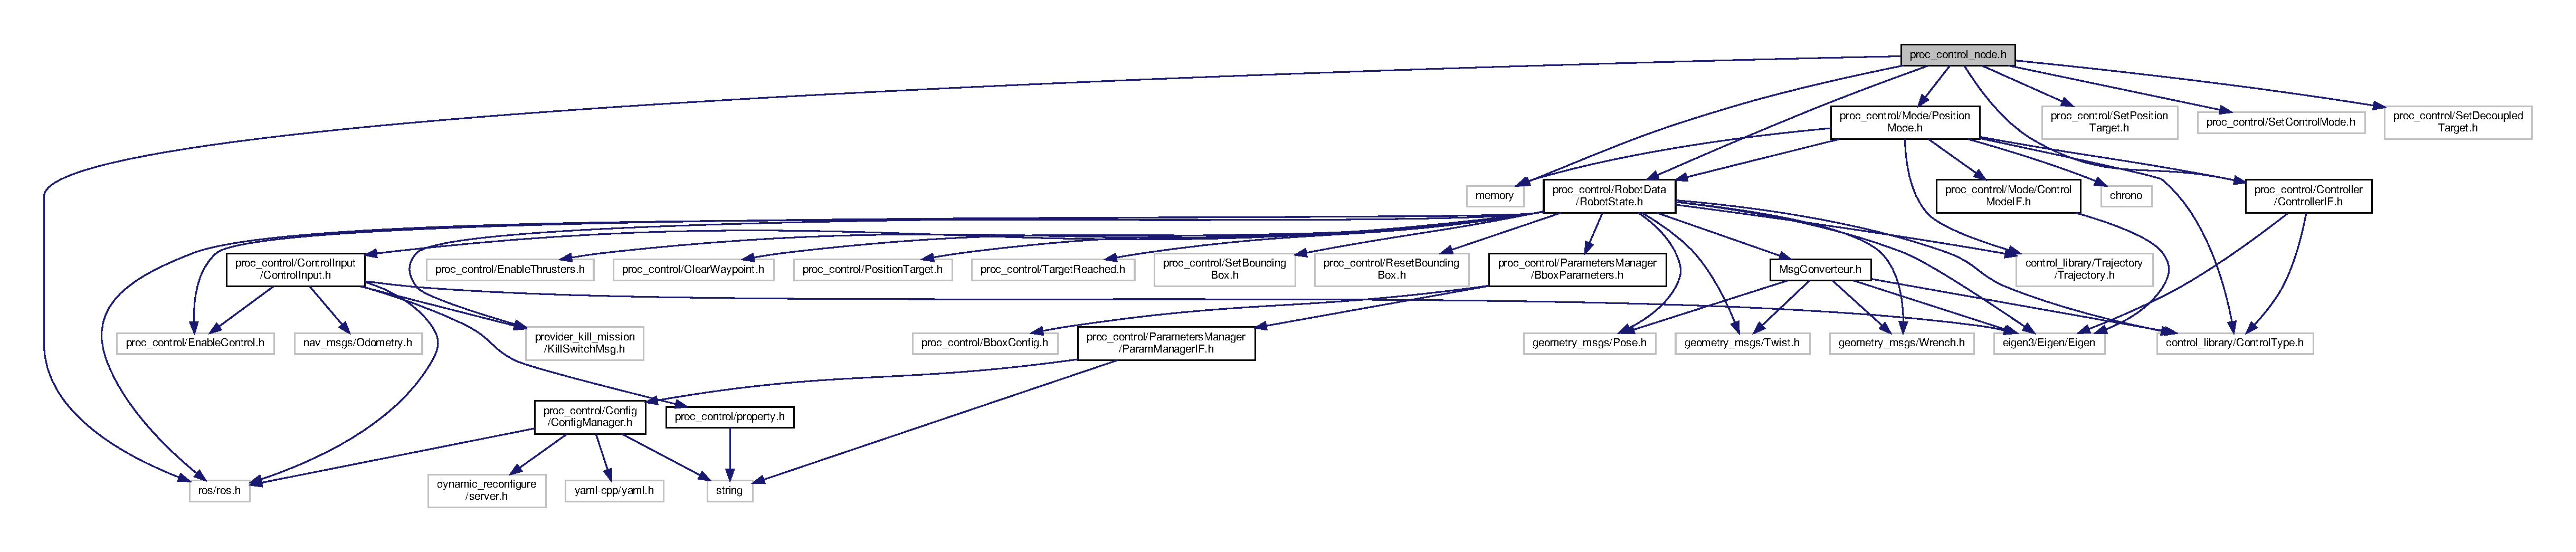
\includegraphics[width=350pt]{proc__control__node_8h__incl}
\end{center}
\end{figure}
This graph shows which files directly or indirectly include this file\+:\nopagebreak
\begin{figure}[H]
\begin{center}
\leavevmode
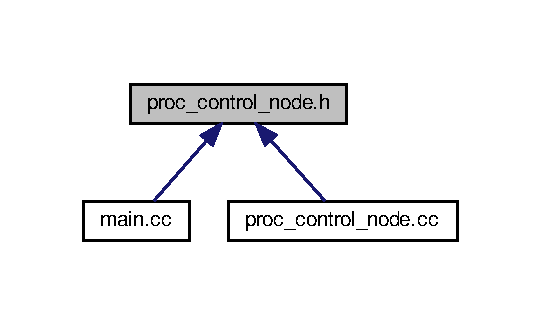
\includegraphics[width=260pt]{proc__control__node_8h__dep__incl}
\end{center}
\end{figure}
\subsection*{Classes}
\begin{DoxyCompactItemize}
\item 
class \hyperlink{classproc__control_1_1_proc_control_node}{proc\+\_\+control\+::\+Proc\+Control\+Node}
\end{DoxyCompactItemize}


\subsection{Detailed Description}
\begin{DoxyAuthor}{Author}
Olivier Lavoie \href{mailto:olavoie9507@gmail.com}{\tt olavoie9507@gmail.\+com} 
\end{DoxyAuthor}
\begin{DoxyDate}{Date}
10/21/17
\end{DoxyDate}
\begin{DoxyCopyright}{Copyright}
Copyright (c) 2017 S.\+O.\+N.\+I.\+A. A\+UV All rights reserved.
\end{DoxyCopyright}
\hypertarget{property_8h_LICENSE}{}\subsection{L\+I\+C\+E\+N\+SE}\label{property_8h_LICENSE}
This file is part of S.\+O.\+N.\+I.\+A. software.

S.\+O.\+N.\+I.\+A. A\+UV software is free software\+: you can redistribute it and/or modify it under the terms of the G\+NU General Public License as published by the Free Software Foundation, either version 3 of the License, or (at your option) any later version.

S.\+O.\+N.\+I.\+A. A\+UV software is distributed in the hope that it will be useful, but W\+I\+T\+H\+O\+UT A\+NY W\+A\+R\+R\+A\+N\+TY; without even the implied warranty of M\+E\+R\+C\+H\+A\+N\+T\+A\+B\+I\+L\+I\+TY or F\+I\+T\+N\+E\+SS F\+OR A P\+A\+R\+T\+I\+C\+U\+L\+AR P\+U\+R\+P\+O\+SE. See the G\+NU General Public License for more details.

You should have received a copy of the G\+NU General Public License along with S.\+O.\+N.\+I.\+A. A\+UV software. If not, see \href{http://www.gnu.org/licenses/}{\tt http\+://www.\+gnu.\+org/licenses/}. 
\hypertarget{property_8h}{}\section{property.\+h File Reference}
\label{property_8h}\index{property.\+h@{property.\+h}}
{\ttfamily \#include $<$string$>$}\newline
Include dependency graph for property.\+h\+:\nopagebreak
\begin{figure}[H]
\begin{center}
\leavevmode
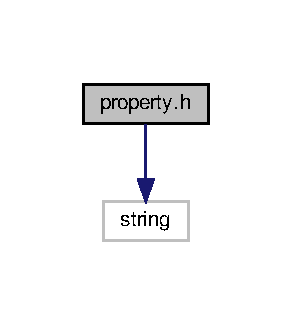
\includegraphics[width=140pt]{property_8h__incl}
\end{center}
\end{figure}
This graph shows which files directly or indirectly include this file\+:\nopagebreak
\begin{figure}[H]
\begin{center}
\leavevmode
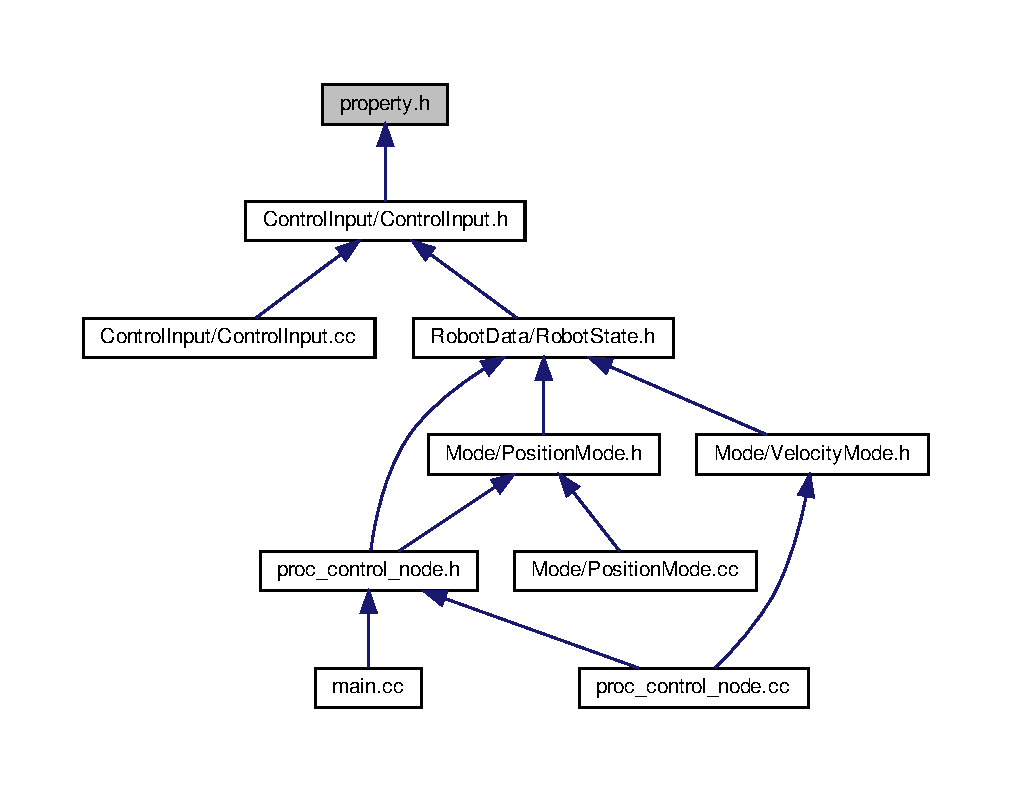
\includegraphics[width=350pt]{property_8h__dep__incl}
\end{center}
\end{figure}
\subsection*{Variables}
\begin{DoxyCompactItemize}
\item 
\mbox{\Hypertarget{property_8h_a68cf5fea512727a0fbb62b558806c3c1}\label{property_8h_a68cf5fea512727a0fbb62b558806c3c1}} 
const std\+::string {\bfseries k\+Node\+Name} = \char`\"{}/proc\+\_\+control/\char`\"{}
\item 
\mbox{\Hypertarget{property_8h_af953190bfe09191220bd3575b48c3ead}\label{property_8h_af953190bfe09191220bd3575b48c3ead}} 
const std\+::string {\bfseries k\+Project\+Folder\+Path} = std\+::getenv(\char`\"{}R\+O\+S\+\_\+\+S\+O\+N\+I\+A\+\_\+\+WS\char`\"{})
\item 
\mbox{\Hypertarget{property_8h_ad49938ab28b6f7e5f9c35f110fbb5661}\label{property_8h_ad49938ab28b6f7e5f9c35f110fbb5661}} 
const std\+::string {\bfseries k\+Project\+Path} = k\+Project\+Folder\+Path + \char`\"{}/src\char`\"{} + k\+Node\+Name
\item 
\mbox{\Hypertarget{property_8h_afb7b8f6b780fc7e694f6d3e2518bd150}\label{property_8h_afb7b8f6b780fc7e694f6d3e2518bd150}} 
const std\+::string {\bfseries k\+Config\+Path} = k\+Project\+Path + \char`\"{}config/\char`\"{}
\item 
\mbox{\Hypertarget{property_8h_a7adb0ba85632ab52d9a045eb226cba83}\label{property_8h_a7adb0ba85632ab52d9a045eb226cba83}} 
const std\+::string {\bfseries k\+Config\+Ext} = \char`\"{}.yaml\char`\"{}
\item 
\mbox{\Hypertarget{property_8h_ab2ce89e06bf93c79ecbf61b36b4658d3}\label{property_8h_ab2ce89e06bf93c79ecbf61b36b4658d3}} 
const size\+\_\+t {\bfseries X} = 0
\item 
\mbox{\Hypertarget{property_8h_a112d438ef5f2ea76a8a154cee2f309e9}\label{property_8h_a112d438ef5f2ea76a8a154cee2f309e9}} 
const size\+\_\+t {\bfseries Y} = 1
\item 
\mbox{\Hypertarget{property_8h_aef46543dd4e4165b2e7decb928628bde}\label{property_8h_aef46543dd4e4165b2e7decb928628bde}} 
const size\+\_\+t {\bfseries Z} = 2
\item 
\mbox{\Hypertarget{property_8h_a0b30a8d3df3bec8de793cabe32d84e87}\label{property_8h_a0b30a8d3df3bec8de793cabe32d84e87}} 
const size\+\_\+t {\bfseries R\+O\+LL} = 3
\item 
\mbox{\Hypertarget{property_8h_a33dde2ba01238d9f9148eddbc532bf05}\label{property_8h_a33dde2ba01238d9f9148eddbc532bf05}} 
const size\+\_\+t {\bfseries P\+I\+T\+CH} = 4
\item 
\mbox{\Hypertarget{property_8h_ad04db1cb686a759abcee818e81f2852e}\label{property_8h_ad04db1cb686a759abcee818e81f2852e}} 
const size\+\_\+t {\bfseries Y\+AW} = 5
\end{DoxyCompactItemize}


\subsection{Detailed Description}
\begin{DoxyAuthor}{Author}
Jeremie St-\/\+Jules-\/\+Prevost \href{mailto:jeremie.st.jules.prevost@gmail.com}{\tt jeremie.\+st.\+jules.\+prevost@gmail.\+com} 
\end{DoxyAuthor}
\begin{DoxyDate}{Date}
2016
\end{DoxyDate}
\begin{DoxyCopyright}{Copyright}
Copyright (c) 2017 S.\+O.\+N.\+I.\+A. All rights reserved.
\end{DoxyCopyright}
This file contains all the constants properties for the proc control.\hypertarget{_robot_state_8h_LICENSE}{}\subsection{L\+I\+C\+E\+N\+SE}\label{_robot_state_8h_LICENSE}
This file is part of S.\+O.\+N.\+I.\+A. software.

S.\+O.\+N.\+I.\+A. A\+UV software is free software\+: you can redistribute it and/or modify it under the terms of the G\+NU General Public License as published by the Free Software Foundation, either version 3 of the License, or (at your option) any later version.

S.\+O.\+N.\+I.\+A. A\+UV software is distributed in the hope that it will be useful, but W\+I\+T\+H\+O\+UT A\+NY W\+A\+R\+R\+A\+N\+TY; without even the implied warranty of M\+E\+R\+C\+H\+A\+N\+T\+A\+B\+I\+L\+I\+TY or F\+I\+T\+N\+E\+SS F\+OR A P\+A\+R\+T\+I\+C\+U\+L\+AR P\+U\+R\+P\+O\+SE. See the G\+NU General Public License for more details.

You should have received a copy of the G\+NU General Public License along with S.\+O.\+N.\+I.\+A. A\+UV software. If not, see \href{http://www.gnu.org/licenses/}{\tt http\+://www.\+gnu.\+org/licenses/}. 
%--- End generated contents ---

% Index
\backmatter
\newpage
\phantomsection
\clearemptydoublepage
\addcontentsline{toc}{chapter}{Index}
\printindex

\end{document}
